\chapter{Results and Discussion}

%%%%%%%%%%%%%%%%%%%%%%%%%%%%%%%%%%%%%%%%%%%%%%%%%%%%%%%%%%%%%%%%%%%%%%%%
\section{Final Number}

\begin{comment}
    Measured asymmetry 
    $\downarrow$
    correct for Coulomb distortions 
    $\downarrow$
    Weak density at one $Q^2$
    $\downarrow$
    small correction for $G_E^n$, $G_E^s$
    $\downarrow$
    Neutron density at one $Q^2$
    $\downarrow$
    assume suface thickness good to 25\% (MFT)
    $\downarrow$
    $R_n$

\end{comment}
The overall beam polarization was inverse-variance weighted average of the Complton
and Moller measurements.
\begin{table}[!h]
    % PREX-II Compton
    % PREX-II Moller: https://prex.jlab.org/DocDB/0004/000468/003/DNP_Oct2020.pdf
    % CREX Compton: AJZ thesis
    % CREX Moller: AJZ thesis
    \centering
    \begin{tabular}{c | c c}
	\hline
	    & PREX-II	& CREX	\\
	\hline
	Compton	& ($89.68 \pm 0.15$)\%  & ($87.115 \pm 0.453$)\%	\\
	Moller	& ($89.67 \pm 0.80$)\%	& ($87.06 \pm 0.74$)\%  \\
	\hline
	Average	& ($89.7 \pm 0.8$)\%	& ($87.10 \pm 0.39$)\%	\\
	\hline
    \end{tabular}
    \caption{Beam polarization measured by the Compton and Moller polarimeters.}
\end{table}

%%%%%%%%%%%%%%%%%%%%%%%%%%%%%%%%%%%%%%%%%%%%%%%%
% \subsection{Asymmetry}
After beam false asymmetry correction, we need to remove various background 
asymmetries, and the final physical PV asymmetry will be extracted using 
Eq. \ref{eq:background_correction}, which we restate here 
\begin{equation*}
    \CA_{pv} = \frac{\CA_{cor}/\CP - \sum_i \CA_i f_i}{1 - \sum_i f_i}
\end{equation*}
List of various corrections to our final result is shown in 
Table \ref{tab:prex_corrections} and \ref{tab:crex_corrections}.

\begin{table}
    \centering
    \begin{tabular}{l r@{ $\pm$ }l r@{ $\pm$ }l}
	\hline
	Correction & \multicolumn{2}{c}{Absolute (ppb)}	& \multicolumn{2}{c}{Relative (\%)}   \\
	\hline
	Beam trajectory and energy  & -60.4	& 3.0	& 11.0	& 0.5	\\ 
	Charge correction           & 20.7	& 0.2   & 3.8	& 0.0   \\ 
	\hline
	Beam polarization           & 56.8	& 5.2   & 10.3	& 1.0   \\ 
	Target diamond foils        & 0.7	& 1.4   & 0.1	& 0.3   \\ 
	Spectrometer rescattering   & 0.0	& 0.1   & 0.0  	& 0.0   \\ 
	Inelastic contributions     & 0.0	& 0.1   & 0.0  	& 0.0   \\ 
	Transverse asymmetry        & 0.0	& 0.3   & 0.0  	& 0.1   \\ 
	Detector nonlinearity       & 0.0	& 2.7   & 0.0  	& 0.5   \\ 
	Angle determination         & 0.0	& 3.5   & 0.0  	& 0.6   \\ 
	Acceptance function         & 0.0	& 2.9   & 0.0  	& 0.5   \\ 
	\hline
	Total correction	    & 17.7	& 8.2	& 3.2	& 1.5	\\
	Statistical uncertainty	    & \multicolumn{2}{c}{16}	& \multicolumn{2}{c}{2.9}   \\
	\hline
    \end{tabular}
    \caption{Corrections and corresponding systematic uncertainties to $\CA_{pv}$ in PREX-II.}
    \label{tab:prex_corrections}
\end{table}

\begin{table}
    \centering
    \begin{tabular}{l r@{ $\pm$ }l r@{ $\pm$ }l}
	\hline
	Correction & \multicolumn{2}{c}{Absolute (ppb)}	& \multicolumn{2}{c}{Relative (\%)}   \\
	\hline
	Beam trajectory and energy  & 68  & 7     & 2.5	    & 0.3   \\         
	Beam charge asymmetry       & 112 & 1     & 4.2     & 0.0   \\         
	\hline
	Beam polarization	    & 382 & 13    & 14.3    & 0.5   \\         
	Isotopic purity             & 19  & 3     & 0.7     & 0.1   \\         
	3.831 MeV ($2^+$) inelastic & -35 & 19    & -1.3    & 0.7   \\         
	4.507 MeV ($3^-$) inelastic & 0   & 10    & 0	    & 0.4   \\ 
	5.370 MeV ($3^-$) inelastic & -2  & 4     & -0.1    & 0.1   \\         
	Transverse asymmetry        & 0   & 13    & 0	    & 0.5   \\ 
	Detector nonlinearity       & 0   & 7     & 0	    & 0.3   \\         
	Acceptance                  & 0   & 24    & 0  	    & 0.9   \\         
	Radiative corrections	    & 0   & 10    & 0  	    & 0.4   \\         
	\hline
	Total systematic uncertainty	& \multicolumn{2}{c}{40}    & \multicolumn{2}{c}{1.5}	\\
	Statistical uncertainty		& \multicolumn{2}{c}{106}   & \multicolumn{2}{c}{4.0}	\\
	\hline
    \end{tabular}
    \caption{Corrections and corresponding systematic uncertainties to $\CA_{pv}$ in CREX.}
    \label{tab:crex_corrections}
\end{table}

The last step is unblinding, which is to subtract $\CA_{blind}$ from the blinded
$\CA_{pv}$. The blinding value was just a randomly picked up constant that was unknown to
everyone until the last moment and was added to every true asymmetry values. 
Surprisingly, the PREX-II $\CA_{blind}$ is very close to 0, making the unblinded
$\CA_{phy}$ almost the same as the blinded one. The final asymmetry values are
shown in Table \ref{tab:pcrex_final_number}.
\begin{table}
    \centering
    \begin{tabular}{c | c c}
	\hline
	Asymmetry   & PREX-II	& CREX	\\
	\hline
	$\CA_{raw}$ & $431.64 \pm 44.01$    & $2106 \pm 178.9$	\\
	$\CA_{cor}$ & $492.02 \pm 13.52$    & $2080.3 \pm 83.8$	\\
	Blinded $\CA_{phy}$ & $549.4 \pm 16.1 \pm 8.1$    & $2334.8 \pm 106.1 \pm 37.3$	\\
	$\CA_{blind}$	& -0.5	& -255.7    \\
	\hline
	Unblinded $\CA_{phy}$	& $550 \pm 16 \pm 8$	& $2659 \pm 106 \pm 40$	\\
	\hline
    \end{tabular}
    \caption{The path to a physical PV asymmetry. All values unit in $ppb$.}
    \label{tab:pcrex_final_number}
\end{table}

%%%%%%%%%%%%%%%%%%%%%%%%%%%%%%%%%%%%%%%%%%%%%%%%
\subsection{Neutron Skin Thickness}
With the physical PV asymmetry, we can calculate the weak FF using Eq. \ref{eqn:asymmetry}.
The weak radius is obtained by plotting its correlation with $\CA_{pv}$ predicted
by a series of density functional models, as shown in Fig. \ref{fig:prex_Rw}. The neutron
skin is derived in the same way, as shown by the right axis of Fig. \ref{fig:prex_Rw}.
The results for PREX-II and CREX are summarized in Table \ref{tab:pcrex_neutron_skin}.

The weak charge density we used in predication of various DFT models is the 2-parameter
Fermi function
\begin{equation*}
    \rho_W(r) = \rho_W^0 \frac{\sinh(c/a)}{\cosh(r/a) + \cosh(c/a)}
\end{equation*}
where c denotes the nuclear size while a means the surface thickness. We fit $\rho_W(r)$
from various density functional models to $\rho_W(r, c, a)$ to extract values of
c and a. Then the weak saturation density will be
\begin{equation}
    \rho_W^0 = \frac{3Q_W}{4\pi c (c^2 + \pi^2 a^2)} 
    = -0.0798 \pm 0.0038 (\text(exp)) \pm 0.0013 (\text{theo})\ fm^{-3}
\end{equation}

\begin{figure}
    \centering
    % 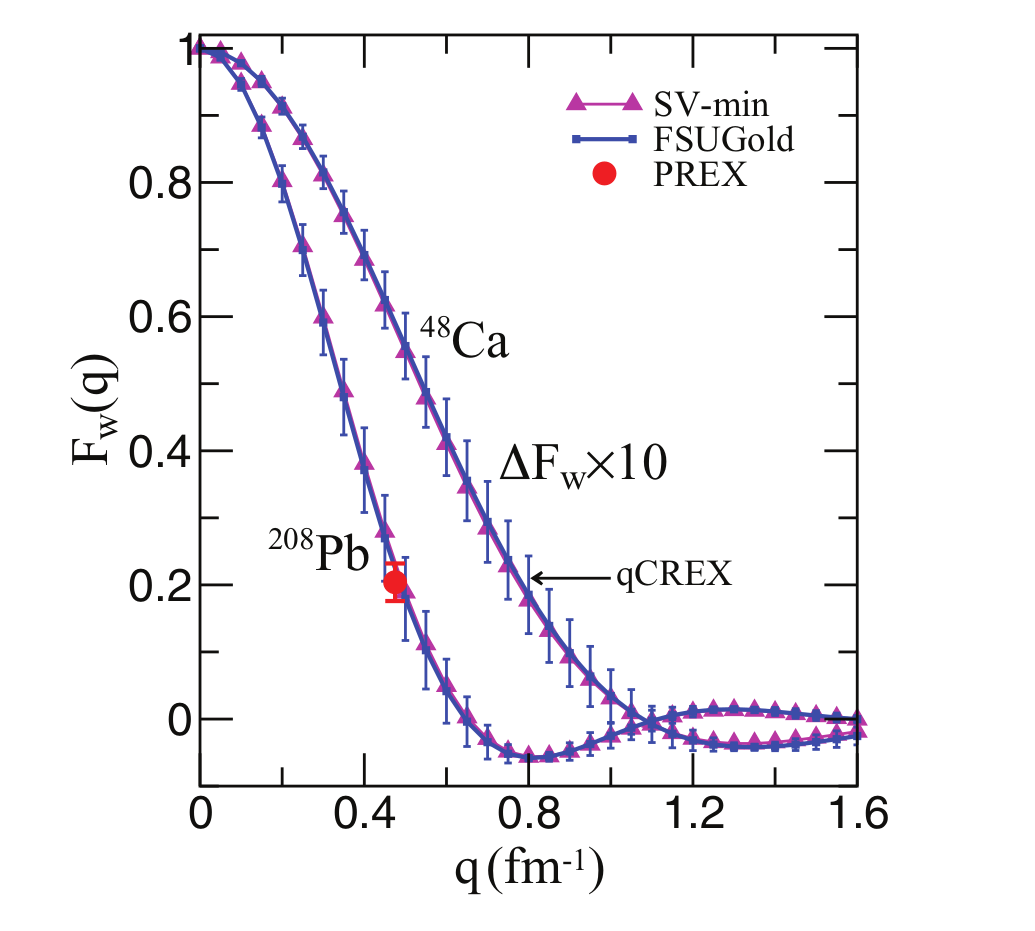
\includegraphics[width=0.6\linewidth]{weak_FF}
    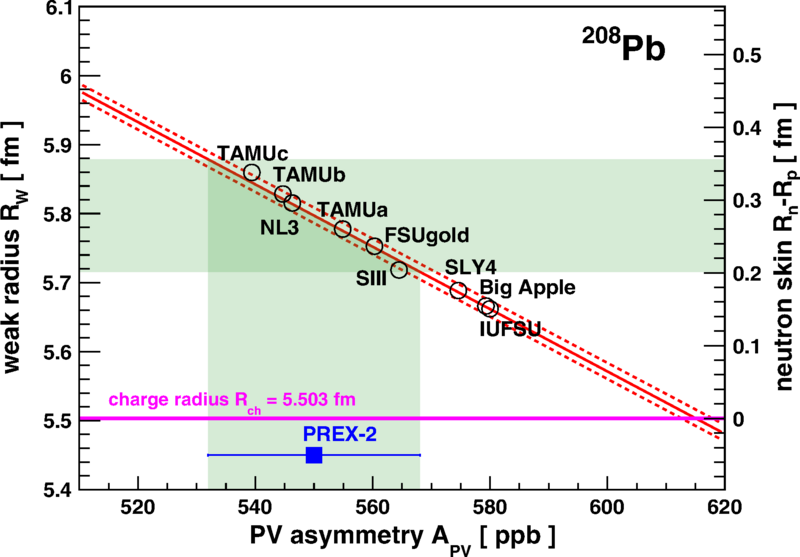
\includegraphics[width=0.6\linewidth]{prex_Rw}
    \caption{Correlation between weak radius (neutron skin thickness) with $\CA_{pv}$ for \Pb.}
    \label{fig:prex_Rw}
\end{figure}

\begin{table}[!h]
    \centering
    \begin{tabular}{l | c c}
	\hline
	Exp.	& PREX-II   & CREX  \\
	\hline
	Target	& \Pb	    & \Ca   \\
	$\langle Q^2 \rangle $ ($GeV^2$)	& $ 0.00616 \pm 0.00005 $   & $0.0297 \pm 0.0002 $  \\
	$\langle \CA_{pv} \rangle$ ($ppb$)   & $550 \pm 16 (\text{stat}) \pm 8 (\text{syst})$	& $2668 \pm 106 (\text{stat}) \pm 40 (\text{syst})$ \\
	$F_W$	& $0.368 \pm 0.013 (\text{exp}) \pm 0.001 (\text{theo})$    & $0.1304 \pm 0.0052 (\text{stat}) \pm 0.0020 (\text{syst})$    \\
	$F_{ch} - F_W$	& $0.041 \pm 0.013 (\text{exp}) \pm 0.001 (\text{theo})$    & $0.0277 \pm 0.0052 (\text{stat}) \pm 0.0020 (\text{syst})$    \\
	$R_w$ ($fm$)	& $5.795 \pm 0.082 (\text{exp}) \pm 0.013 (\text{theo})$    &	\\
	$R_n - R_p$ ($fm$)  & $0.278 \pm 0.078 (\text{exp}) \pm 0.012 (\text{theo})$	& $0.121 \pm 0.026 (\text{exp}) \pm 0.024 (\text{theo})$    \\
	$\rho_W^0$ ($fm^{-3}$)	& $-0.0798 \pm 0.0038 (\text{exp}) \pm 0.0013 (\text{theo})$	&   \\
	$\rho_b^0$ ($fm^{-3}$)	& $0.1482 \pm 0.0040 $	&   \\
	\hline
    \end{tabular}
    \caption{Physical results extracted from PREX-II and CREX.}
    \label{fig:pcrex_neutron_skin}
\end{table}
% the 0.28 fm neutron skin thickness of Pb208 is larger than the predicted
% value of 0.15-0.18 fm by most models. Such a thin neutron skin indicates
% a strong symmetry pressure, therefore a larger neutron star radius.
%%%%%%%%%%%%%%%%%%%%%%%%%%%%%%%%%%%%%%%%%%%%%%%%%%%%%%%%%%%%%%%%%%%%%%%%
\section{Physical Implication}

%%%%%%%%%%%%%%%%%%%%%%%%%%%%%%%%%%%%%%%%%%%%%%%%
\subsection{Nuclear Structure}
\begin{comment}
    QCD ==> EFT ==> Interactions ==> ab-initio ==> shell model ==> DFT
\end{comment}
Unlike particle physics, there is no such a single Standard Model to describe
static properties and dynamics of atomic nuclei, such as the ground state binding energy,
nuclear size and excitation spectrum. 
The fundamental building blocks of nuclei are quarks and gluons, theoretically, 
all properties of a nucleus can be derived directly from interactions
of these elementary particles using Quantum ChromoDynamics (QCD). 
Many groups do work in this direction, trying to figure out nuclear structure from QCD 
directly. Unfortunately, it turns out to be a very hard job and only limited advance
was achieved. At the low energy scale where nuclei lie in, the non-perturbative nature of 
QCD makes the problem so complicated that even the state-of-the-art lattice QCD
technique can resolve only small nuclear system with a few nucleons.
So quarks and gluons are not the right degrees of freedom to describe nuclei, up
to now.

% first problem: nuclear forces governed by QCD, which is non-perturbative at 
% low energy
Instead of quarks and gluons, the more natural choice of degrees of freedom for
description of a nuclear system are nucleons and their intermedia particle pions.
This was how physicists study a nuclear system in the beginning (1930's \cite{10.1143/PTPS.1.1,}). 
Many nuclear models were developed based on meson-exchange phenomenology, called
phenomenological interactions, up to the mid 1990's.
With the uncovering of QCD, this approach was re-discovered from the aspect of QCD:
quarks and gluons are confined in colorless nucleons and pions, the nuclear force
is just the residual interaction between quarks and gluons. So it is appropriate
to describe nuclear systems in terms of nucleons and pions.

%%%%%%%%%%%%%%%%%%%%%%%%
\subsubsection{Ab-initio Method}
Though we don't know how nuclear force emerges from the underlying QCD interaction,
they should share the same properties, especially the same symmetries and symmetry-breaking
patterns. % among which, the most important one is the spontaneously broken chiral symmetry.
Placed on this idea, in 1990's, S. Weinberg proposed a new framework: the chiral 
effective field theory ($\chi$EFT), which is an effective realization of the 
underlying QCD Lagrangian based on chiral symmetry \cite{WEINBERG}.

% All possible terms that are consistent with the underlying QCD symmetry.

Ab-initio methods try to calculate the wave function of nuclei by solving the
many-body Schr\"{o}dinger equation:
\begin{equation}
    H\ket{\psi} = E\ket{\psi}
\end{equation}
where the Hamiltonian is
\begin{equation}
    H = T + V = \frac{1}{A} \sum_{i<j}^A \frac{(\vec{p}_i - \vec{p}_j)^2}{2m} 
	+ \sum_{i<j}^A V_{ij}^{NN} + \sum_{i<j<k}^A V_{ijk}^{NNN} + \cdots
\end{equation}

$\chi$EFT requires that the potential should follow the same symmetries of QCD,
like spacetime translation, rotation, parity transformation, etc. Most importantly, V should
preserve the spontaneously broken chiral symmetry. Constrained by these symmetries,
the potential operator takes the form of
\begin{equation}
    \mathds{O}_V = \{\mathds{1}, \vec{\sigma}_i \cdot \vec{\sigma}_j, \vec{L} \cdot \vec{S}, S_{ij}\} 
	\times \{\mathds{1}, \vec{\tau}_i \cdot \vec{\tau}_j\}
\end{equation}
where $\vec{\sigma}_i \cdot \vec{\sigma}_j$ ($\vec{\tau}_i \cdot \vec{\tau}_j$) term
denote spin (isospin) interaction, 
$\vec{L} \cdot \vec{S}$ indicates the spin-orbit interaction and tensor interaction
is represented by 
$S_{ij}(\vec{x}) = 3(\vec{\sigma} \cdot \hat{\vec{x}})(\vec{\sigma}_j \cdot \hat{\vec{x}}) - \vec{\sigma}_i \cdot \vec{\sigma}_j$.

The typical momentum (soft scale) in nuclei is $p \sim m_\pi \sim \mathds{O}(100\ MeV)$, while the
short-range structure involves heavier meson (hard scale) is about 
$\Lambda_\chi \sim m_\rho \sim \mathds{O}(700 \ MeV)$. 
The clear gap between the soft and hard scale allows the seperation of long-range force 
from the short-range one. Effective means we will consider only the pion excahnge
in low-energy scale, while heavier mesons will be integrated out as low-energy
constants (LECs) and phenomenologically fitted. 
\begin{figure}[H]
    \centering
    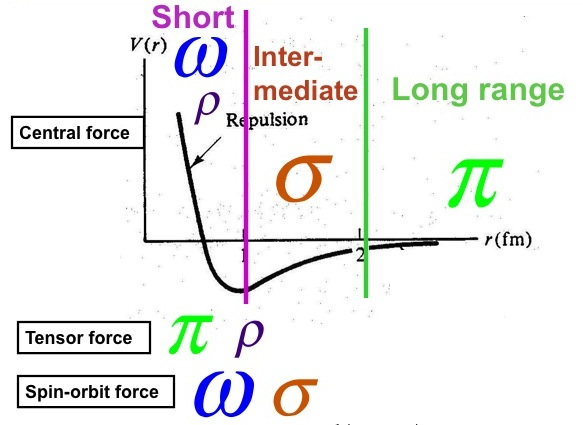
\includegraphics[width=0.5\linewidth]{nuclear_force}
    \caption{Seperation of nuclear potential.}
\end{figure}
With this low-energy approximation, one can expand the potential in terms of
$\left(\frac{Q}{\Lambda_\chi}\right)^\nu$, where Q is the momentum transfer
between 2 nucleons and $\Lambda_\chi$ is the cut off scale where short-range 
interactions becomes important, and
finally $\nu$ is the power, defining the order of interactions. 
\begin{equation}
    V = \sum_i V^{(i)} = V^{(0)}_{LO} + V^{(2)}_{NLO} + V^{(3)}_{NNLO} + V^{(4)}_{NNNLO} \cdots
\end{equation}
In this way, one can calculate nuclear force to any precision, by including
more higher order terms.

\begin{figure}
    \centering
    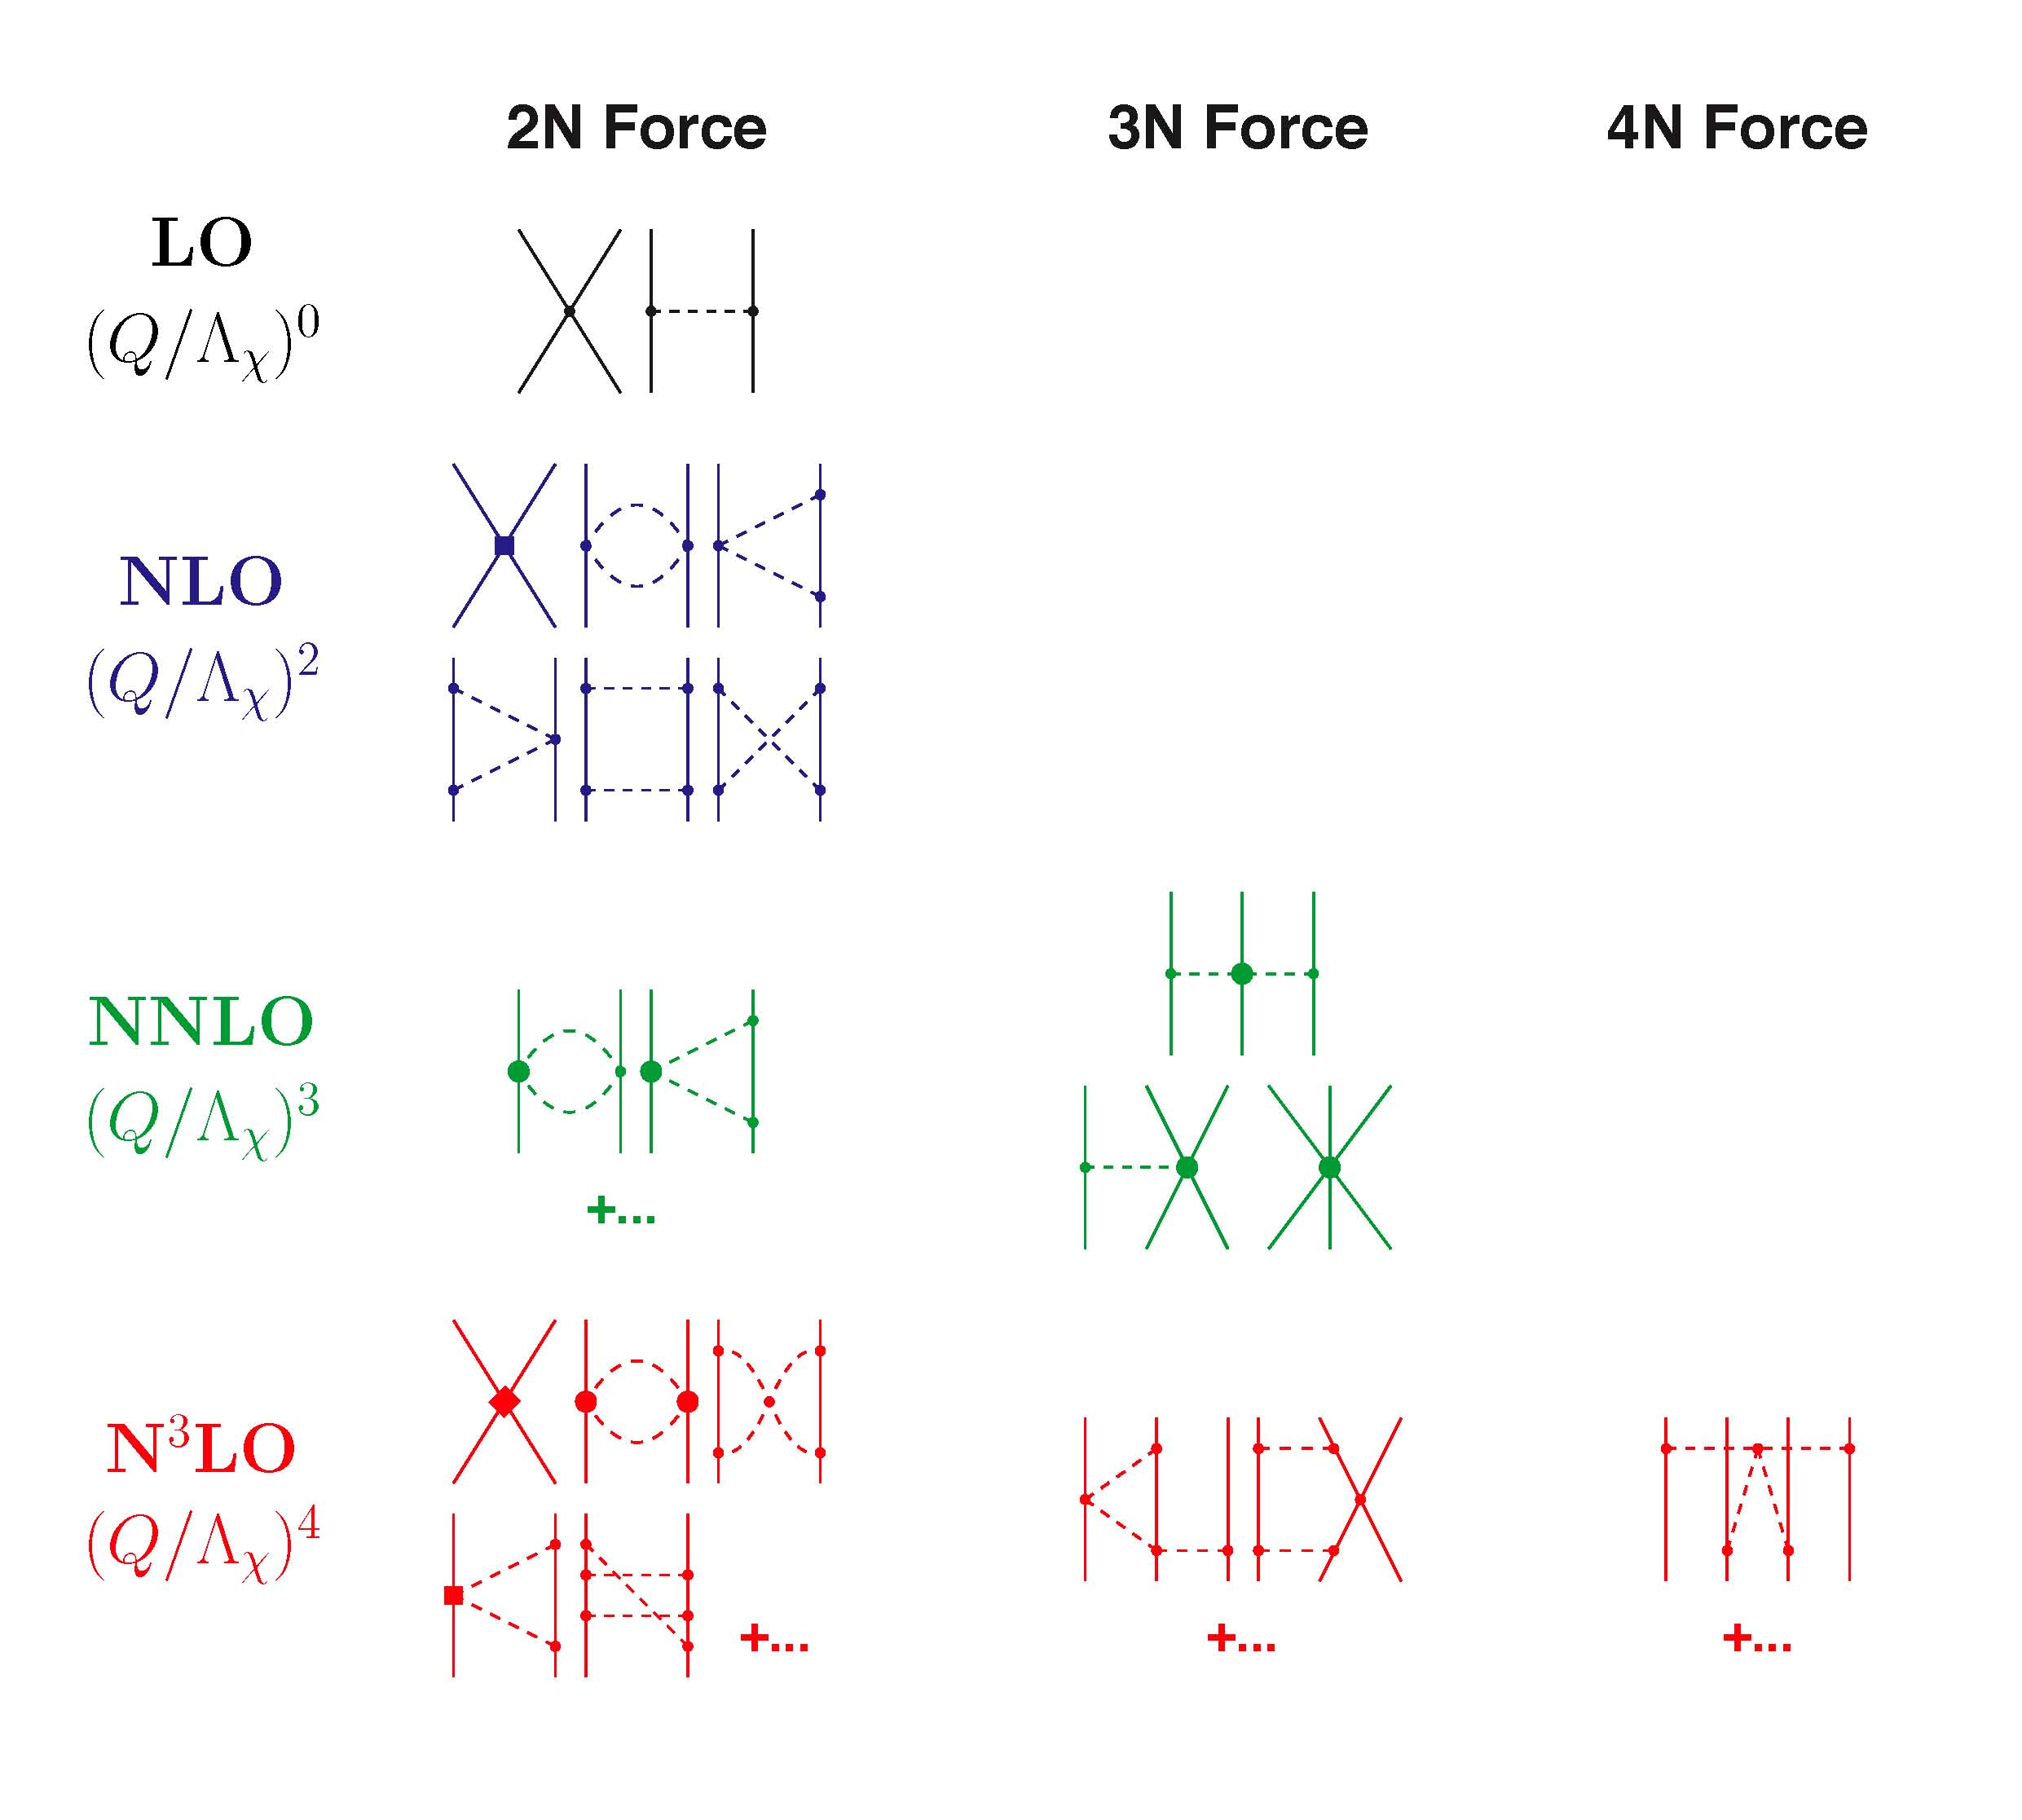
\includegraphics[width=0.5\linewidth]{nuclear_force_diagrams}
    \caption{Feynman diagrams for nuclear interactions.}
\end{figure}

For example, the $1\pi$-exchange potential between 2 nucleons is:
\begin{equation}
    V_{2N}^{1\pi} = -\frac{g_A^2}{4F_\pi^2}
    \frac{(\vec{\sigma}_1\cdot\vec{q})(\vec{\sigma}_2\cdot\vec{q})}{\vec{q}^2 + M^2_\pi}
    \vec{\tau}_1\cdot\vec{\tau}_2 
\end{equation}
where $g_A$ and $f_\pi$ are the axial-vector coupling constant and the pion 
decay constant.

If the nuclear force potential is identified, one can solve the Schr\"{o}dinger 
equation to get eigenstate wave-functions, from which various properties can be extracted. 
With the help of many-body methods, like self-consistent Green's function,
coupled cluster and renormalization group, etc. ab-initio method can be extented
to nuclei of multiple nucleons.

\begin{figure}
    \centering
    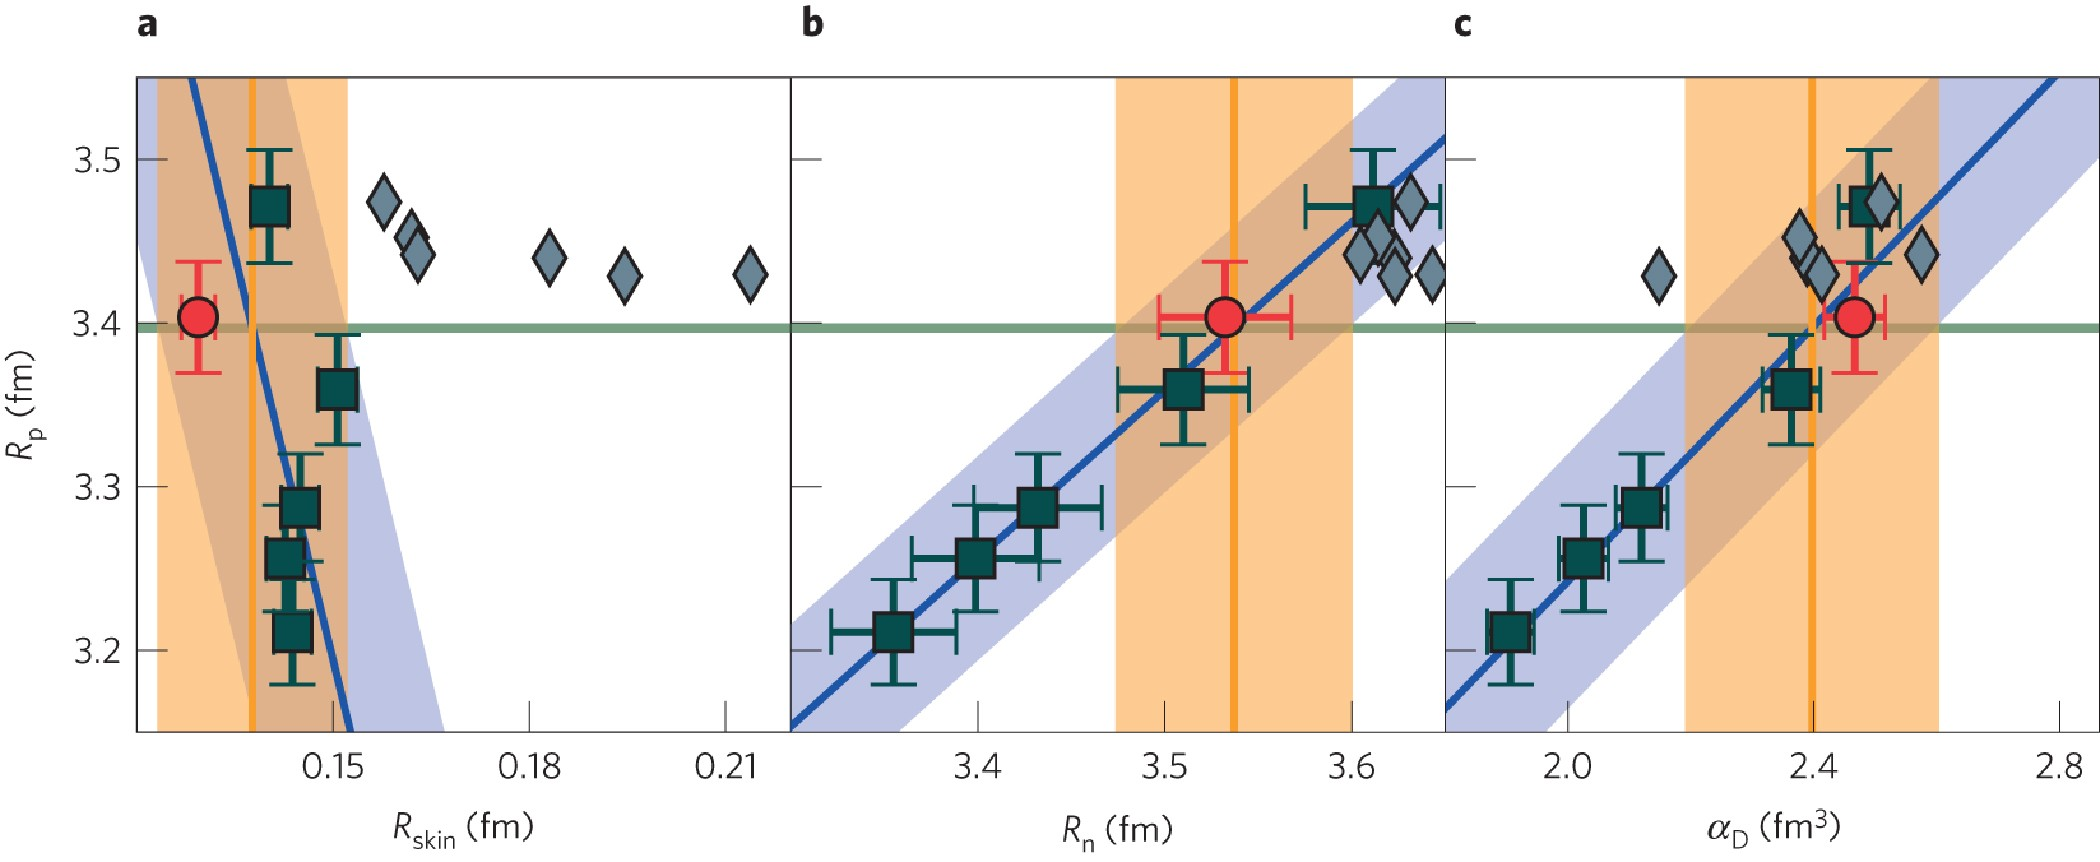
\includegraphics[width=0.8\linewidth]{ab_initio-Ca48_1}
\end{figure}

\begin{comment}
Deviation of ab-initio result and observation for heavy nuclei indicates the 
importance of higher-order interactions.

\begin{equation}
    \CL_{eff} = \CL_{\pi\pi} + \CL_{\pi N} + \CL_{NN} + \cdots
\end{equation}

3-neutron forces are hard to observe directly, they increase the pressure of
neutron matter and therefore the neutron skin thickness of both \Pb and \Ca.

3-nucleon force term
\begin{itemize}
    \item Long-range two-pion exchange
    \item Medium-range one-pion exchange
    \item Short range three-nucleon contact
\end{itemize}
\end{comment}
%%%%%%%%%%%%%%%%%%%%%%%%
\subsubsection{Nuclear Density Functional Theory (DFT)}
% The second problem is many-body problem
Though of the ab-initio's success in light and some medium nuclei, it is still 
unable to deal with heavy nuclei due to limitation of computation resource.
Instead of building the nuclear theory bottom up, one may do it the opposite
way, start from nuclear phenomenologies, and try to go back to the underlying
QCD. The method developed in this way is the DFT method.

The DFT method originated from solid-state physics, to deal with many-electron
problem in solid-states, it lays its foundation on the Hohenberg
and Kohn (HK) theorem \cite{PhysRevC.57.3430}. The idea is that one can write
the system's total energy based on the fermion (electron) density (density functional), 
then the minimization of this density functional leads to the ground state 
density distribution. In this way, one can greatly reduce the number of DOF, 
from 3N to 3. The only problem is that HK theorem 
doesn't tell us how to construct such a density functional.

In the case of nuclear interaction, it is more complicate than the Coulomb interaction, 
because 3-nucleon interaction is not negligible. Fortunately, the nuclear interaction
is short-range interaction. Given the experimental fact that the nucleon mean
free path in nuclei is about or larger than the nuclear radius, which means
nucleons don't experience nuclear interaction frequently. This valids the use
of mean-field method, namely nucleons move in a one-body potential which averages 
over interactions with all other nucleons. The most famous one is the Woods-Saxon
potential.

As 
\begin{equation}
    H = \sum_i^N -\frac{\hbar^2}{2m}\nabla_i^2 + \frac{1}{2} \sum_{i\neq j=1}^N V(i, j)
\end{equation}

\begin{equation}
    E_{HF}(\rho) = \bra{\Phi} H \ket{\Phi}
\end{equation}
where $\ket{\Phi}$ is the Slater determinant made up with single-particle wave 
function $\ket{\phi}$

\begin{equation}
    \frac{\delta}{\delta\rho(\vec{r})} \left( E_{HF} - \epsilon\int d^3r' \phi^*_j(\vec{r}')\phi_j(\vec{r}') \right) = 0
\end{equation}

Because 
\begin{equation}
    \rho(\vec{r}) = \sum_i^N \phi_i^*(\vec{r})\phi_i(\vec{r})
\end{equation}
we will get the well-known HF equations:
\begin{equation}
    \begin{aligned}
	-\frac{\hbar^2}{2m}\nabla^2\phi_j(\vec{r}) 
	+ \sum_{l=1}^N \int d^3\vec{r}' \phi^*_l(\vec{r}') V(\vec{r}, \vec{r}') (\phi_l(\vec{r}')\phi_j(\vec{r}) - \phi_l(\vec{r}')\phi_l(\vec{r}'))
	&= \epsilon_j\phi_j(\vec{r})	\\
	\bra{j}\frac{-\hbar^2}{2m}\nabla^2\ket{j} + \sum_{l=1}^N \bra{jl}V(1-P_{12})\ket{jl} = \epsilon_j
    \end{aligned}
\end{equation}
where $P_{12}$ exchanges particles 1 and 2. This leads to the total energy
\begin{equation}
    E_{HF} = T + \frac{1}{2}\sum_{jl} \int d^3r d^3r' \phi_j^*(\vec{r}')\phi_;^*(\vec{r}')V(\vec{r}, \vec{r}') (\phi_j(\vec{r}')\phi_l(\vec{r}') - \phi_l(\vec{r}')\phi_j(\vec{r}'))
\end{equation}
here T is the kinematic energy.

By knowing the interaction (potential term), one will be able to calculate density
distribution and therefore total energy of the system and other properties. One
successful model is the Skyrme force

\begin{equation}
    \begin{aligned}
	V_{Skyrme}(\vec{r}_1, \vec{r}_2) &= t_0 (1 + x_0 P_\sigma)\delta(\vec{r}_1 - \vec{r}_2) 
	+ \frac{1}{2}t_1 (1 + x_1 P_\sigma) \left( \vec{k}^{\dag2}\delta(\vec{r}_1 - \vec{r}_2) + \delta(\vec{r}_1 - \vec{r}_2)\vec{k}^2 \right)    \\
	&+ t_2(1 + x_2 P_\sigma)\vec{k}^\dag \cdot \delta(\vec{r}_1 
	    - \vec{r}_2)\vec{k} + \frac{1}{6} t_3 (1 + x_3 P_\sigma)\delta(\vec{r}_1 - \vec{r}_2) \rho^\alpha\left( \frac{\vec{r}_1 + \vec{r}_2}{2} \right) \\
	&+ iW_0 (\vec{\sigma}_1 + \vec{\sigma}_2) \cdot \vec{k}^\dag \times \delta(\vec{r}_1 - \vec{r}_2) \vec{k}
    \end{aligned}
\end{equation}
which has up to 10 parameters that are constrained by experimental data, like
nuclear mass, radius and binding energy.

\begin{comment}
DFT is actually also an ab-initio method, the key distinction lies in the
exchange-correclation functional, some DFT models have its parameters fitted
to empirical data, but most reliable result are based on first-principles.

The basic idea is simple, once we know the density distribution function, then
one can calculate the total energy of the system based on this distribution 
function, minimization of the total energy will be the ground state, and other
static properties will be inferred from the ground state. Excitation properties
can also be calculated from DFT. The only problem is how to know the density
distributio function.
\end{comment}

\begin{figure}
    \centering
    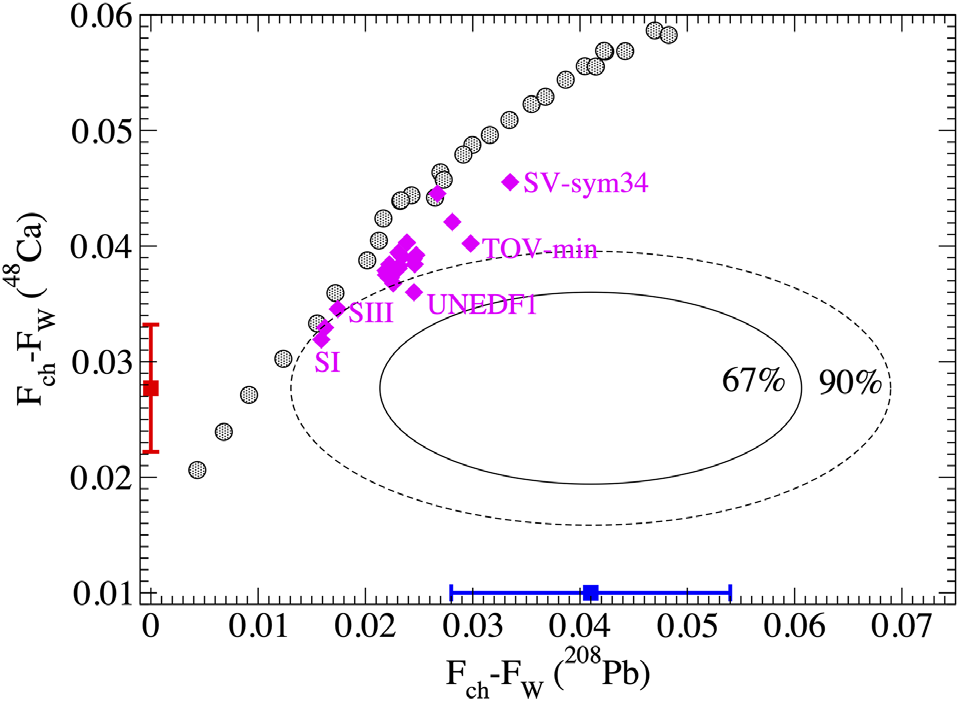
\includegraphics[width=0.49\linewidth]{FF_difference_Ca48_vs_Pb208}
    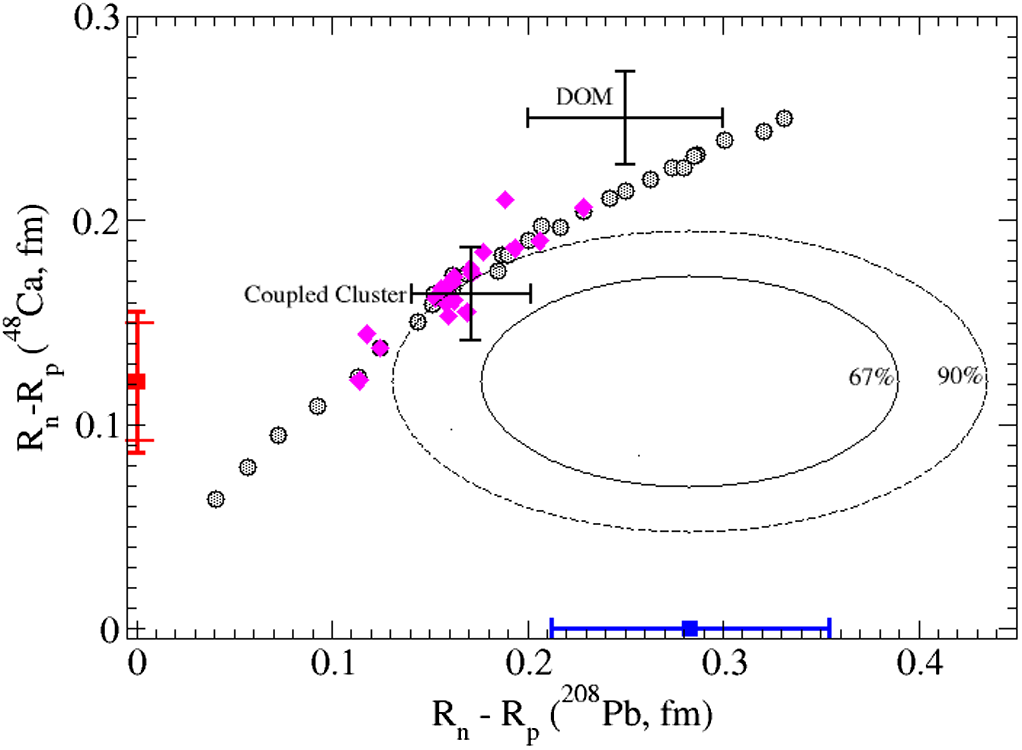
\includegraphics[width=0.49\linewidth]{neutron_skin_Ca48_vs_Pb208}
\end{figure}


\begin{comment}
% The strength of an EFT approach to thenuclear force lies in its power-counting capability. That is, theLagrangian of a theory with nucleons and pions can be expanded  order  by  order  in  terms  of  momentum  transfer  divided by a parameter that sets the momentum scale of the expansion
Various EFT models are based on an effective interacting Lagragian, for example,
FSUGold model has the following effective Lagrangian \cite{PhysRevLett.95.122501}:
\begin{equation}
    \begin{aligned}
	\CL_{\text{int}} = &\bar{\psi} \left[ g_s\phi - \left( g_v V_\mu + \frac{g_\rho}{2}\vec{\tau}\cdot\vec{b}_\mu + \frac{e}{2}(1 + \tau_3) A_\mu \right)\gamma^\mu \right]\psi \\
	    & - \frac{\kappa}{3!}(g_s\phi)^3 - \frac{\lambda}{4!}(g_s\phi)^4 + \frac{\zeta}{4!}(g_v^2 V_\mu V^\mu )^2	\\
	    & + \Lambda_v(g_\rho^2\vec{b}_\mu\vec{b}^\mu)(g_v^2 V_\mu V^\mu)
    \end{aligned}
\end{equation}
This Lagrangian density descirbes interactions of the nucleon field $\psi$ to
various meson fields and their self-interctions. $\phi$ is a scalar.

The difference between different EFT models is just how many coupling they
include in their effetive Lagrangian density. With the Lagrangian density,
one can calculate the properties of various nuclei, fitting predicted values
to experimental results to get a parameter set for the coupling constant in
the Lagrangian, which is called one model. Frequently used EFT models include
NL3 \cite{}, FSUGold \cite{} and 
\end{comment}

%%%%%%%%%%%%%%%%%%%%%%%%
\subsubsection{Limit of Nuclear Landscape}
One straightforward application of DFT is to identify limits of the nuclear
landscape. Every year, as many as dozens or as few as several new nuclides
are discovered \cite{NEW_NULCIDES}. A clear guidence from the theory part
about the possible area of neutron-rich nuclei will help a lot in finding 
new rare isotopes, given the experimental fact that the production rate of 
neutron-rich nuclei is very low.

The possible atomic nucleus in the nuclear chart is bounded by the 
`drip line', which determines the maximum number of protons (neutrons) for a 
given number of neutrons (protons). More physically, across the drip line, the
seperation energy of one proton ($S_{1p}$) or neutron ($S_{1n}$) 
or two protons ($S_{2p}$) or neutrons ($S_{2n}$) change sign (from positive to negative).
Surprisingly, the neutron drip line is known only up to neon ($Z=10$), with the 
maximum number of neutron as $N=24$ \cite{PhysRevLett.123.212501}. 
% https://physics.aps.org/articles/v15/177#c1

\begin{figure}
    \centering
    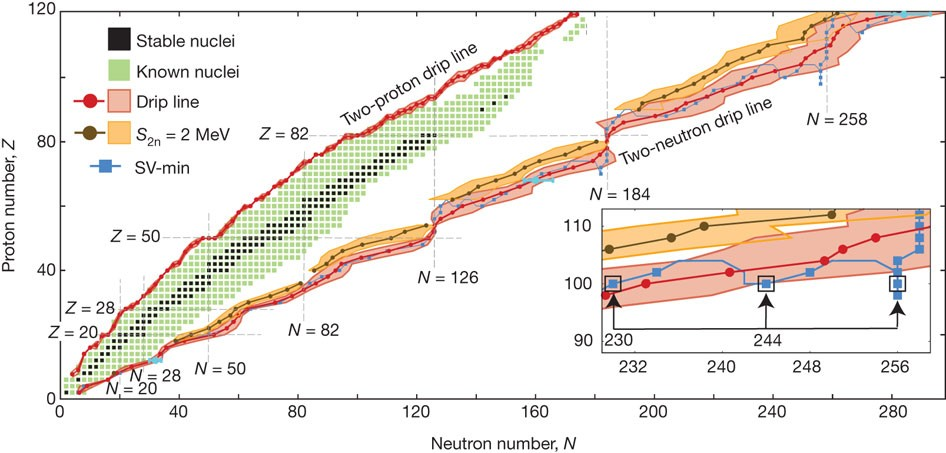
\includegraphics[width=0.8\linewidth]{nuclear_landscape_2012}
    \caption{Nuclear even-even landscape as of 2012 \cite{Erler2012}}
\end{figure}

The seperation energy is defined as:
\begin{equation}
    \begin{aligned}
	S_{1n}(Z, N) &= E(Z, N-1) - E(Z, N) \\
	S_{2n}(Z, N) &= E(Z, N-2) - E(Z, N) \\
    \end{aligned}
\end{equation}
where E is the binding energy, the same definition for proton seperation energy.
When the seperation energy is positive, the nucleus is bounded, otherwise unstable.
We concern both $S_{1n}$ and $S_{2n}$, rather than $S_{1n}$ only, because nuclei
with even-numbers of nucleons are more stable than their neighbors of odd-numbers
of nucleons, due to nucleonic superfluidity. Currently, the estimation of the
neutron drip line depends on the choice of theoretical models and corresponding
parameterizations, as shown in Fig. \ref{fig:neutron_drip_line}. By constraining
DFT models with PREX-II and CREX result, we can improve the robustness of theoretical
prediction of the neutron drip line.
\begin{figure}
    \centering
    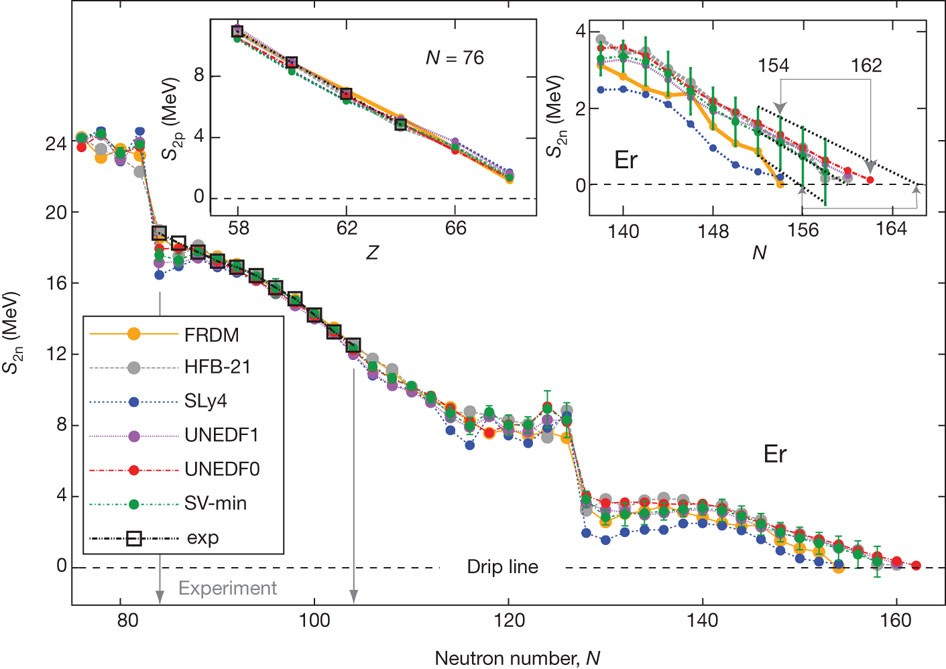
\includegraphics[width=0.8\linewidth]{drip_line}
    \caption{Theoretical and Experimental two-nucleon seperation energies of
    even-even erbium isotopes \cite[Erler2012]. Various dots represent DFT calculations.}
    \label{fig:neutron_drip_line}
\end{figure}

%%%%%%%%%%%%%%%%%%%%%%%%
\subsubsection{Nuclear Saturation Density}
% for A > 20, B/A ~ constant (8 MeV)
The invariance of bingding energy per nucleon ($E_b/A$) w.r.t. A means that
the interaction between nucleons is not proportional to $A(A-1)$, but proportional
to A, which means nucleons saturate, in other word, the interior baryon density 
is approximatively constant. A more strict definition of the saturation density
is the density where binding energy is minimized.

Though of the knowledge of nuclear saturation, it is never directly observed.
\ca is the largest stable $N=Z$ nucleus, but still too small to have nearly 
constant interier baryon density. For heavy nuclei, charge density of those
nuclei exist, but no interior neutron or baryon density. PREX-II is the first
experiment to provide a clean value of average interior baryon density of a heavy nucleus.

Using 2-parameter Fermi function \cite{PhysRevC.102.044321}, we extract the 
weak charge saturation density.
\begin{equation}
    \rho_{wk}(r, c, a) = \rho^0_{wk} \frac{\sinh(c/a)}{\cosh(r/a) + \cosh(c/a)}
\end{equation}

\begin{equation}
    R^2_{wk} = \frac{1}{Q_{wk}}\int r^2 \rho_{wk}(r)d^3r = \frac{3}{5}c^2 + \frac{7}{5}(\pi a)^2
\end{equation}

\begin{equation}
    \rho^0_{wk} = \frac{27 Q_{{wk}}}{4\pi(5R^2_{wk} - 4\pi^2 a^2)\sqrt{15R^2_{wk} - 21\pi^2 a^2}}
\end{equation}
Take average thickness from theory
\begin{equation}
    a = 0.605 \pm 0.025\ fm
\end{equation}

\begin{figure}
    \centering
    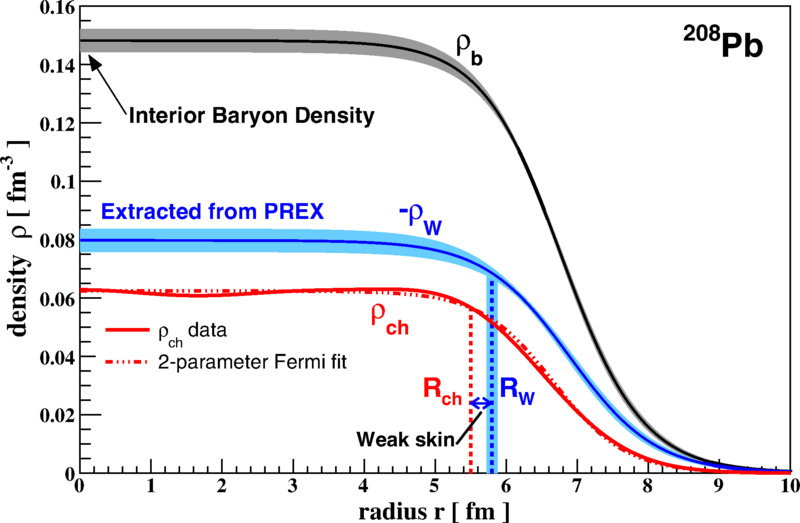
\includegraphics[width=0.6\linewidth]{prex_baryon_density}
\end{figure}

The baryon saturation density is measured to be
\begin{equation}
    \rho^0_b = 0.1482 \pm 0.0040\ fm^{-3}
\end{equation}


\begin{comment}
%%%%%%%%%%%%%%%%%%%%%%%%%%%%%%%%%%%%%%%%%%%%%%%%
\subsection{Atomic Parity Violation Asymmetry}
Atomic parity violation is caused by the exchange of $Z^0$ boson between electrons
and the quarks in the nucleus, which interferes with the ``normal'' Coulomb interaction.

The exchange of a $Z^0$ boson is a parity violating effect and it causes the atomic states 
to acquire a small admixture of opposite-parity states. The effect is dominated by 
the admixture of P states into S states, $S \rightarrow S + \epsilon P$. 
In this case a parity-forbidden electric quadropole E2 $S \rightarrow D$ transition 
is joined by an E1 parity non-conserving transition. The parity mixing effect is tiny, 
but it has been shown (Bouchiat \& Bouchiat, 1974) that it scales faster than $Z^3$, 
so the effect will be larger for heavier atoms.

Accuracy of atomic PV measurement is about 0.3\% (FIXME), which is important
for the test of the SM and the search for physics beyond the SM. A higher (0.1\%)
precision requires knowledge about the neutron radius better than 1\%. \cite{PhysRevC.46.2587}

\begin{equation}
    H_{PNC} \approx \frac{G_F}{2\sqrt{2}}\int [-N\rho_N(\vec{r}) + Z(1-4\sin^2\theta_W)\rho_P(\vec{r})] \phi_e^\dag \gamma^5\phi_e d^3r
\end{equation}

%%%%%%%%%%%%%%%%%%%%%%%%%%%%%%%%%%%%%%%%%%%%%%%%
\subsection{Coherent Neutrino Scattering off Nucleus}
\begin{equation}
    \frac{d\sigma}{dT} \approx \frac{G_F^2 M}{2 \pi}\frac{Q^2_W}{4}F^2(Q)\left ( 2 - \frac{MT}{E_\nu^2} \right)
\end{equation}
where E is the neutrino energy and T is the nuclear recoil energy. M being the
nuclear mass and $Q=\sqrt{2MT}$ is the momentum transfer.

\begin{itemize}
    \item neutrino floor for dark matter searches
    \item high precision determination of nuclei allow coherent neutrino 
	scattering to probe non-standard neutrino interactions.
\end{itemize}
\end{comment}

%%%%%%%%%%%%%%%%%%%%%%%%%%%%%%%%%%%%%%%%%%%%%%%%
\subsection{Neutron Stars}
As we discussed in the introduction section, in spite of the great difference
in their size, the neutron star and the neutron skin in neutron-rich nuclei
share the same nuclear EoS. So by probing the neutron skin thickness of \Pb and
\Ca, the result will remind us the stiffness of the EoS, which can be used to
constraint the size of neutron stars.

% some extreme properties
Neutron star is the most dense celestial body known, the pressure is so strong
that even atoms inside the star collapse, crushing together electrons
and protons into neutrons, that's why the name of neutron star. Primarily neutron
stars are observed either as pulsars or in binary systems. By exploring
neutron stars, we will touch some fundermental questions in nuclear physics and 
astrophysics. Like
\begin{itemize}
    \item What are the high density phase of QCD?
    \item WHat is the structure of many compact and energetic objects in the heavens
	and what determines their EM, neutrino and gravitational-wave radiations.
\end{itemize}

Specifically, the connection between the neutron skin thickness and the size of
a neutron star is the pressure. It is the same pressure that supports the neutron
skin against the surface tension and a neutron star against gravity. 
The larger the neutron skin thickness, the larger the pressure, and therefore 
the larger the radius of the neutron star; vice versa.
% Pb neutron skin constrains the pressure of neutron matter at subnuclear densities
% while NS radius depends on the pressure at nuclear density and above

Neutron star is expected to have a solid crust over the liquid core. The phase transition
from high density core to low density crust depends on the properties of
neutron-rich matter, specifically, the symmetry energy dependence on density L.
A thickner neutron skin in \Pb indicates a large value of L, or rapid rise of
symmetry energy with density, which leads to a low transition density in neutron
star.

PREX-II measures L to be
\begin{equation}
    L = 106 \pm 37 \ MeV
\end{equation}

One can also learn about direct UCRA cooling of neutron stars from the
neutron skin thickness of \Pb. Proton fraction for matter in beta equilibrium 
depends on symmetry energy. So the larger neutron skin thickness in \Pb, the
lower the threshold mass for direct URCA cooling. If $R_{skin} > 0.25\ fm$, then
all neutron star models have UCRA cooling process in $1.4 M_{\odot}$ stars.
% some neutron stars seem too cold
%%%%%%%%%%%%%%%%%%%%%%%%
\subsubsection{Multi-Messenger Measurements of Neutron Star Ridius}
NICER (Neutron star Interior Composition ExploreR) is a X-ray telescope that
measures the lightcurve of a neutron star (pulsar). A pulsar has a hot-spot, which
is the magnetic pole of the neutron star. The observed light flux fluctuates 
with the orientation of the hot-spot. When it faces you, you will observe the 
maximum flux; when it eschews you, you will observe the minimum flux due to 
curvature of the space caused by the neutron star. So by observing 
the depth of the light flux, one can infer the curvature of the space near the
neutron star, which depends on the radius of the neutron star. This is how NICER
measures the radius of a neutron star.
\begin{figure}[H]
    \centering
    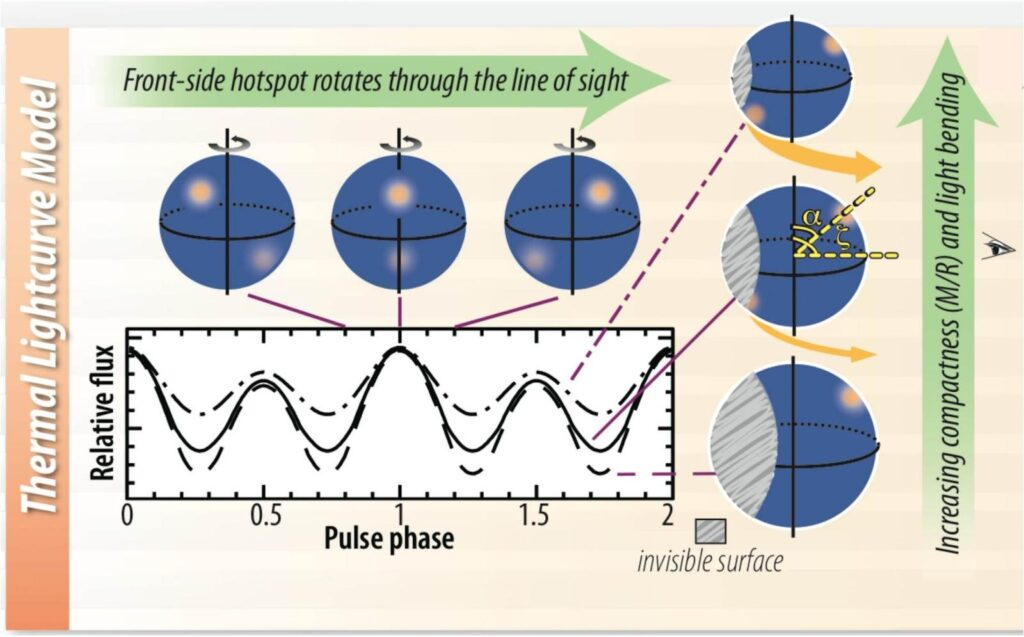
\includegraphics[width=0.6\linewidth]{pulsar_lightcurve}
\end{figure}

One can also measure the size of a neutron star through gravitational waves.
The famous LIGO-Virgo event, GW170817, observed the gravitational wave emission 
from a binary neutron star merger. In a binary system, neutron star deforms
due to tidal force from the other body, this property is described by 
tidal deformability (quadrupole polarizability):
\begin{equation}
    \Lambda = \sum_f \frac{|\bra{f}r^2Y_{20}\ket{i}|^2}{E_f - E_i} \propto R^5 
\end{equation}
Tidal deformability can be probed by detection of gravitational waves.
LIGO observation of GW170817 sets upper limit on $\Lambda$, it favors smaller 
deformability ($<600$) and therefore smaller neutron radius ($<13\ km$)

\begin{figure}
    % page 12 of https://indico2.riken.jp/event/3082/contributions/17269/attachments/10634/15080/PREX2SPIN2021_DonJones.pdf
    \centering
    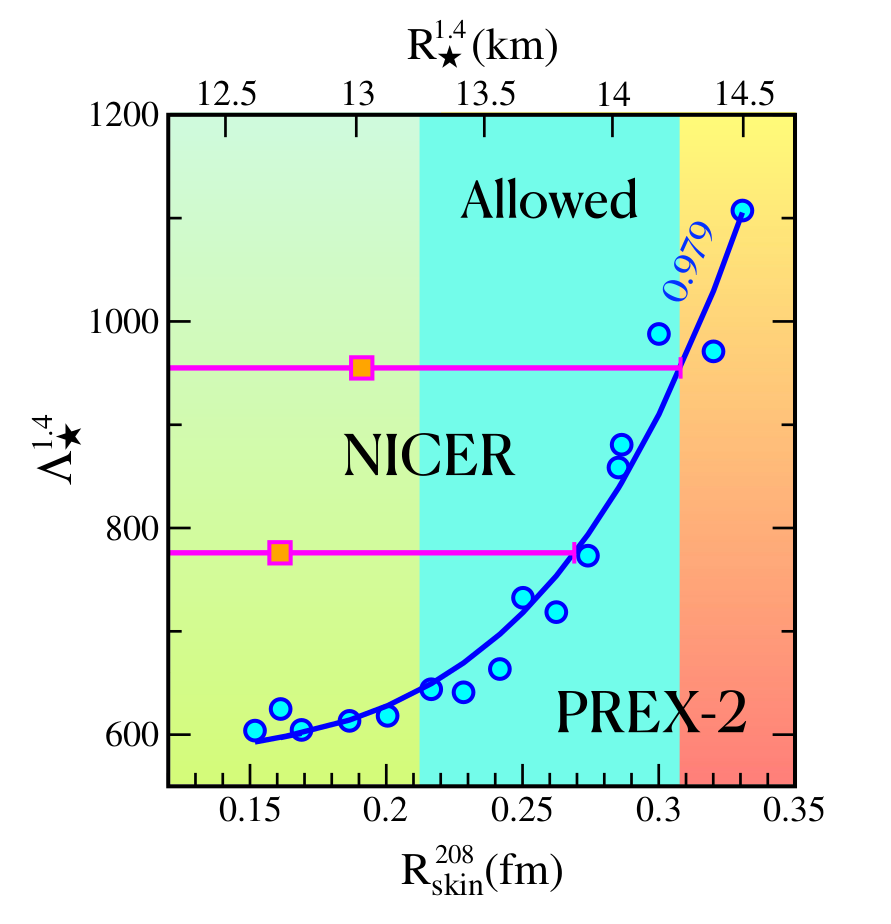
\includegraphics[width=0.6\linewidth]{neutron_star_radius}
    \caption{LIGO sets upper limit on tidal deformability $\Lambda_{1.4} < 580$ 
    for the neutron star merger GW170817: $\Lambda_{1.4} = 190 ^{+390}_{-120}$ (90\% CL).
    Plot from \cite{PhysRevLett.126.172503}}
\end{figure}

The NICER result is consistent with both LIGO observation and PREX-II measurement,
while PREX-II result is a little tensioned with LIGO observation.
% PREX-II result suggests EoS is still at low density while NICER and LIGO observations
% indicate that EoS is soft at high density.
% The softening of EoS with density could strongly suggest a transition to an
% exotic high density phase such as quark matter, starnge matter, color superconductor
% and kaon condensate

\begin{comment}
    \item Dipole polarizability of an atom $\sim R^3$
	$$ \kappa = \sum_f \frac{|\bra{f}rY_{10}\ket{i}|^2}{E_f - E_i} \propto R^3 $$
    \item Tidal deformability (quardupole polarizability) of a neutron star scales as $R^5$
	$$ \Lambda = \sum_f \frac{|\bra{f}r^2Y_{20}\ket{i}|^2}{E_f - E_i} \propto R^5 $$
    \item Next generation observer: cosmic explorer (https://arxiv.org/abs/2109.09882)
	can accurately determine deformability of neutron stars
\end{comment}

%%%%%%%%%%%%%%%%%%%%%%%%
\subsubsection{URCA Cooling}
proton fraction for matter in beat equilibrium depends on symmetry energy S(n).o
The larger Rn in Pb, the lower the threshold mass for direct URCA cooling.
If $R_n - R_p < 0.2 \ fm$ all EOS models don't have direct URCA in 1.4 $M_{sun}$ stars
If $R_n - R_p > 0.25 \ fm$, all models do have URCA in 1.4 $M_{sun}$ stars
\begin{figure}
    \centering
    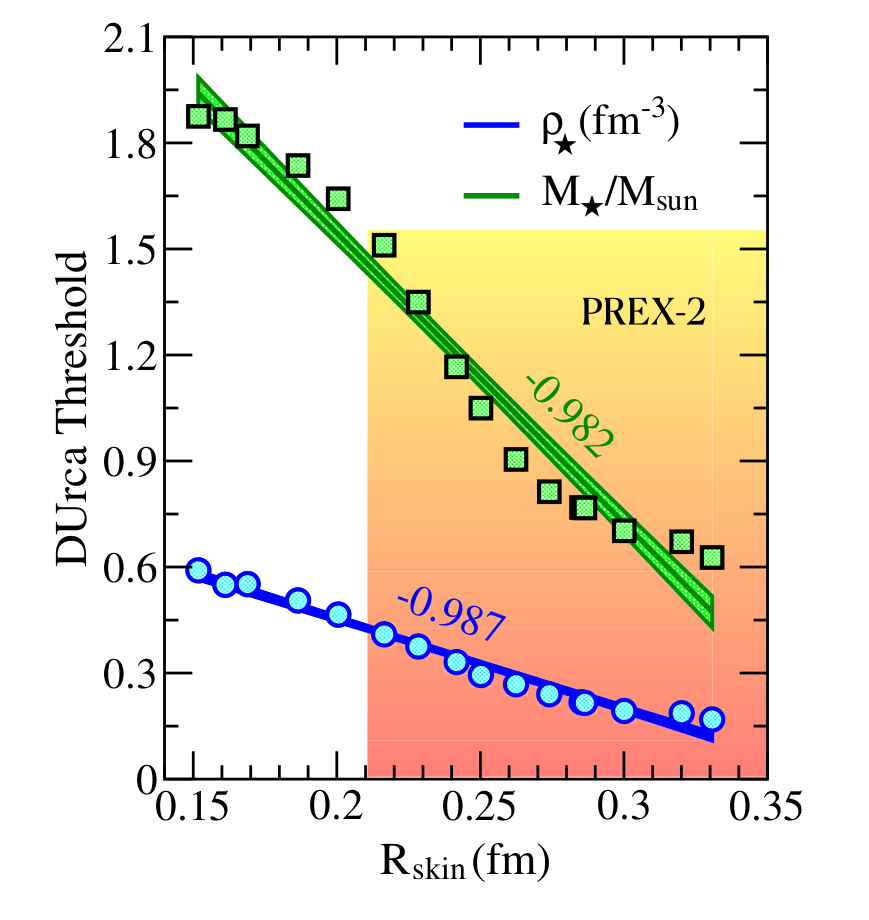
\includegraphics[width=0.5\linewidth]{UCRA_vs_R_skin}
\end{figure}

%%%%%%%%%%%%%%%%%%%%%%%%%%%%%%%%%%%%%%%%%%%%%%%%%%%%%%%%%%%%%%%%%%%%%%%%
\section{Future Outlook}
The PV electron scattering experiments are still developing and flourishing, 
such experiments that will happen in the near future include
MOLLER and the P2 experiments.

%%%%%%%%%%%%%%%%%%%%%%%%
\subsubsection{Measurement Of a Lepton Lepton Electroweak Reaction (MOLLER)}
As a test of the SM, the weak mixing angle ($\sin^2\theta_W$) is of great importance 
and has been measured by SLAC E158 through polarized electron-electron (Moller) scattering:
\begin{equation}
    \CA_{pv} \approx 280 \ ppb
\end{equation}
The proposed MOLLER experiment at JLab in 12 GeV era is a follow up experiment 
of E158, intenting to improve the measurement precision by a factor of 5.
This low energy precison frontier experiment will produce the most precise 
measurement of $\sin^\theta_W$ over the next decade. With such high precision,
the result will be sensitive to interference of the known EM amplitude and any
possible unknown neutron currents, probing new particles beyond the Higgs up
to a scale of $\sim 27\ TeV$.

At tree level, the weak charge of an electron is
\begin{equation}
    Q_W^e = 1 - 4\sin^2\theta_W
\end{equation}
However, $Q_W^e$ runs with energy if one takes into account higher order correction
\begin{figure}
    \centering
    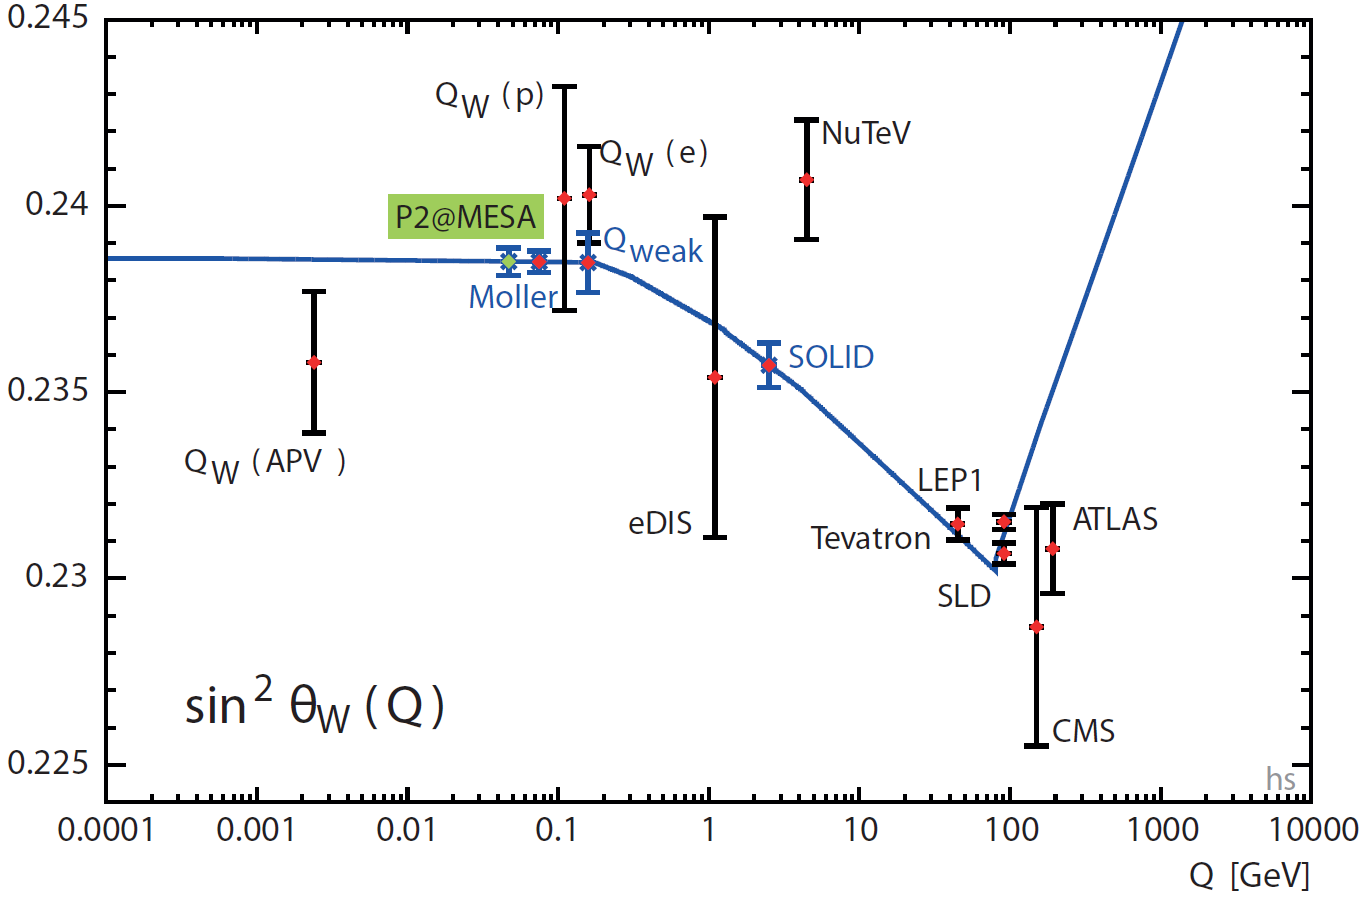
\includegraphics[width=0.5\linewidth]{weak_mixing_angle}
    \caption{Running weak charge (weak mixing angle) along energy scale.}
\end{figure}
Moller will use the upgraded $11\ GeV$ longitudinally polarized electron beam 
to scatter off unpolarized electrons (liquid $H_2$ target), the PV asymmetry
is measured to be
\begin{equation}
    \CA_{pv} = \frac{\sigma_R - \sigma_L}{\sigma_R + \sigma_L}
    = mE\frac{G_F}{\sqrt{2}\pi\alpha}\frac{4\sin^2\theta}{(3+\cos^2\theta)^2} Q_W^e
\end{equation}
where $\theta$ is the scattering angle in the CoM frame. SB Predicts $\CA_{pv} \approx 33 \ ppb$
for Moller kinematics and the overall uncertainty is designed to be $\sigma(\CA_{pv}) = 0.7 \ ppb (2.1\%)$,
which corresponding to $2.4\%$ relative uncertainty in the measurement of $Q_W^e$.
% scattering angle, Q2

% Moller asymmetry: $\CA_{pv} = 35.6 \ ppb$, $\delta(\CA_{pv}) = 0.73\ ppb$, $\delta(Q_W^e) = \pm 2.1\% (stat.) \pm 1.0\% (syst.)$, $\delta(\sin^2\theta_W) = \pm 0.00026 (stat.) \pm 0.00012 (syst.)$

%%%%%%%%%%%%%%%%%%%%%%%%
\subsubsection{Mainz MESA P2}
While MOLLER will be the most precise weak mixing angle measurement, the most
precise weak charge measurement will be the P2 experiment at Mainz.
P2 is also a successor, which will measure the weak charge of proton $Q_W^p = 1 - 4\sin^2\theta_W$
that has been measured by the Qweak experiment at Jlab \cite{???}. Compared to
Qweak, P2 will improve the measurement presicion by a factor of 3.
Similar to MOLLER, P2 provide indirect search for new physics up to a mass scale
of $50\ TeV$.

The electron beam that will be used in P2 has a much lower energy as $155\ MeV$, 
the target is also the liquid $H_2$. The elstaically scattered electrons will
be detected in an azimuthally symmetric Chenrenkov detector. The PV asymmetry
of elastic ep scattering is
\begin{equation}
    \CA_{pv} = -\frac{G_F Q^2}{4\pi\alpha\sqrt{2}} \left[ Q_W^p + F(\theta, Q^2) \right]
\end{equation}
\begin{figure}
    \centering
    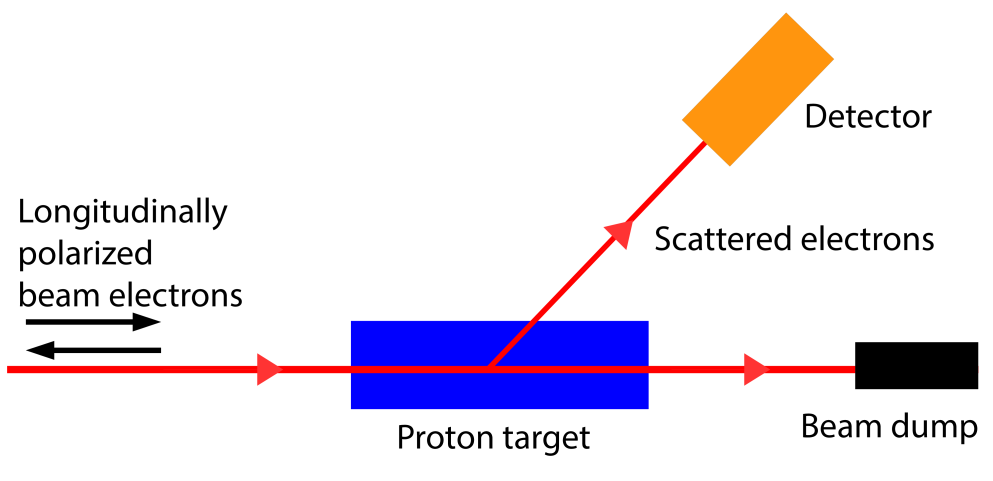
\includegraphics[width=0.5\linewidth]{P2}
\end{figure}
At the selected low $Q^2 \sim 0.006 \ GeV^2$ region, P2 will measure the asymmetry
to a precision of $1.4\%$:
\begin{equation}
    \CA_{pv} = -39.94 \pm 0.56\ ppb
\end{equation}
This translate to $0.14\%$ uncertainty in weak mixing angle:
\begin{equation}
    \sin^2_W = 0.23 \pm 0.00033
\end{equation}
